\documentclass[12pt,a4paper]{article}

% ─── Page Layout ───────────────────────────────────────────────────────────────
\usepackage[a4paper, margin=0.8in, headheight=14pt]{geometry}

% ─── Fonts (XeLaTeX) ───────────────────────────────────────────────────────────
\usepackage{fontspec}
\usepackage{unicode-math}
\setmainfont{TeX Gyre Pagella}
\setmonofont[Scale=0.88]{TeX Gyre Cursor}
\setmathfont{Latin Modern Math}

% ─── Packages ──────────────────────────────────────────────────────────────────
\usepackage{xcolor}
\usepackage{colortbl}
\usepackage{titlesec}
\usepackage{enumitem}
\usepackage{tabularx}
\usepackage{booktabs}
\usepackage{array}
\usepackage{amsmath}
\usepackage{tikz}
\usetikzlibrary{shapes.geometric, arrows.meta, positioning, calc, fit, decorations.pathreplacing}
\usepackage{tcolorbox}
\tcbuselibrary{skins, breakable}
\usepackage{hyperref}
\usepackage{fancyhdr}
\usepackage{graphicx}
\usepackage{microtype}
\hyphenpenalty=10000
\exhyphenpenalty=10000
\sloppy
\usepackage{caption}
\usepackage{setspace}
\usepackage{multirow}
\usepackage{tocloft}

% ─── Q&A helper ────────────────────────────────────────────────────────────────
\newcommand{\Q}[1]{\textbf{#1}\par\noindent\ignorespaces}

% ─── Colour Palette ────────────────────────────────────────────────────────────
\definecolor{myred}{RGB}{196,30,58}
\definecolor{mydark}{RGB}{30,30,50}
\definecolor{mygreen}{RGB}{14,120,80}
\definecolor{myteal}{RGB}{0,130,140}
\definecolor{myamber}{RGB}{180,100,0}
\definecolor{mypurple}{RGB}{100,30,160}
\definecolor{mygray}{RGB}{246,247,249}
\definecolor{mgframe}{RGB}{180,185,200}
\definecolor{watermark}{RGB}{145,150,170}
\definecolor{hdrred}{RGB}{250,232,235}
\definecolor{hdrgreen}{RGB}{220,244,233}
\definecolor{hdrteal}{RGB}{220,242,244}
\definecolor{hdramber}{RGB}{253,242,215}
\definecolor{hdrpurple}{RGB}{238,228,255}
\definecolor{hdrgray}{RGB}{238,240,245}
\definecolor{rowalt}{RGB}{250,251,253}

% ─── Section Formatting ────────────────────────────────────────────────────────
\titleformat{\section}
  {\large\bfseries\color{myred}}{\thesection.}{0.5em}{}
  [\vspace{1pt}{\color{myred}\rule{\linewidth}{0.8pt}}]
\titleformat{\subsection}
  {\normalsize\bfseries\color{myteal}}{\thesubsection}{0.5em}{}
\titlespacing*{\section}{0pt}{18pt}{7pt}
\titlespacing*{\subsection}{0pt}{11pt}{4pt}

% ─── Paragraph ─────────────────────────────────────────────────────────────────
\setlength{\parindent}{0pt}
\setlength{\parskip}{4pt}

% ─── TOC Styling ───────────────────────────────────────────────────────────────
\renewcommand{\cfttoctitlefont}{\large\bfseries\color{myred}}
\renewcommand{\cftaftertoctitle}{\par\noindent{\color{myred}\rule{\linewidth}{0.8pt}}}
\setlength{\cftbeforetoctitleskip}{0pt}
\setlength{\cftaftertoctitleskip}{6pt}
\renewcommand{\cftsecfont}{\normalsize\bfseries\color{mydark}}
\renewcommand{\cftsecpagefont}{\normalsize\bfseries\color{mydark}}
\renewcommand{\cftsecleader}{\cftdotfill{\cftdotsep}}
\setlength{\cftbeforesecskip}{7pt}
\renewcommand{\cftsubsecfont}{\small\color{mydark}}
\renewcommand{\cftsubsecpagefont}{\small\color{mydark}}
\setlength{\cftbeforesubsecskip}{3pt}
\setlength{\cftsubsecindent}{1.4em}

% ─── Table helpers ─────────────────────────────────────────────────────────────
\renewcommand{\arraystretch}{1.45}
\setlength{\tabcolsep}{6pt}
\arrayrulecolor{mydark}
\newcolumntype{B}[1]{>{\small\bfseries\raggedright\arraybackslash}m{#1}}
\newcolumntype{Y}{>{\small\raggedright\arraybackslash}X}
\renewcommand{\tabularxcolumn}[1]{m{#1}}

% ─── Header / Footer ───────────────────────────────────────────────────────────
\pagestyle{fancy}
\fancyhf{}
\fancyhead[L]{\small\color{myred}\textbf{OE-EC604A}\;\color{mydark}--- Electronic Measurement \& Instruments}
\fancyhead[R]{\small\color{myteal}\textbf{Module 3 Notes}}
\fancyfoot[C]{\small\color{mydark}\thepage}
\fancyfoot[R]{\small\color{watermark}\textit{\copyright\ Biraj}}
\renewcommand{\headrulewidth}{0.5pt}
\renewcommand{\footrulewidth}{0.3pt}

% ─── Hyperref ──────────────────────────────────────────────────────────────────
\hypersetup{
  colorlinks=true, linkcolor=myteal, urlcolor=myteal,
  pdfauthor={Biraj Sarkar},
  pdftitle={OE-EC604A --- Module 3 Notes}
}

% ─── tcolorbox styles ──────────────────────────────────────────────────────────
\tcbset{
  tikzbox/.style={
    colback=mygray, colframe=mgframe, boxrule=0.6pt, arc=4pt,
    left=8pt, right=8pt, top=6pt, bottom=6pt,
    colbacktitle=mgframe, coltitle=mydark,
    fonttitle=\small\bfseries
  },
  defbox/.style={
    colback=hdrgreen, colframe=mygreen, boxrule=0.8pt, arc=4pt,
    left=9pt, right=9pt, top=6pt, bottom=6pt,
    colbacktitle=mygreen, coltitle=white,
    fonttitle=\small\bfseries
  },
  formulabox/.style={
    colback=hdrteal, colframe=myteal, boxrule=0.8pt, arc=4pt,
    left=9pt, right=9pt, top=7pt, bottom=7pt,
    colbacktitle=myteal, coltitle=white,
    fonttitle=\small\bfseries
  },
  examplebox/.style={
    colback=hdramber, colframe=myamber, boxrule=0.8pt, arc=4pt,
    left=9pt, right=9pt, top=6pt, bottom=6pt,
    colbacktitle=myamber, coltitle=white,
    fonttitle=\small\bfseries
  },
  masonbox/.style={
    colback=hdrpurple, colframe=mypurple, boxrule=0.8pt, arc=4pt,
    left=9pt, right=9pt, top=6pt, bottom=6pt,
    colbacktitle=mypurple, coltitle=white,
    fonttitle=\small\bfseries
  },
  exambox/.style={
    colback=hdrpurple, colframe=mypurple, boxrule=1pt, arc=5pt,
    left=10pt, right=10pt, top=8pt, bottom=8pt,
    colbacktitle=mypurple, coltitle=white,
    fonttitle=\bfseries,
    breakable, title after break={\textbf{Frequently Asked / Viva Questions (contd.)}}}
}
% Make all boxes breakable across pages
\tcbset{breakable}

% ─── TikZ styles ───────────────────────────────────────────────────────────────
\tikzset{
  block/.style={rectangle, draw=myteal, fill=hdrteal,
    text width=2.1cm, align=center, minimum height=0.95cm,
    font=\small, rounded corners=3pt, line width=0.7pt},
  redblock/.style={rectangle, draw=myred, fill=hdrred,
    text width=2.1cm, align=center, minimum height=0.95cm,
    font=\small, rounded corners=3pt, line width=0.7pt},
  greenblock/.style={rectangle, draw=mygreen, fill=hdrgreen,
    text width=2.1cm, align=center, minimum height=0.95cm,
    font=\small, rounded corners=3pt, line width=0.7pt},
  amberblock/.style={rectangle, draw=myamber, fill=hdramber,
    text width=2.1cm, align=center, minimum height=0.95cm,
    font=\small, rounded corners=3pt, line width=0.7pt},
  purpblock/.style={rectangle, draw=mypurple, fill=hdrpurple,
    text width=2.1cm, align=center, minimum height=0.95cm,
    font=\small, rounded corners=3pt, line width=0.7pt},
  sumjunc/.style={circle, draw=myamber, fill=hdramber,
    minimum size=0.62cm, font=\small, line width=0.8pt},
  arrow/.style={-Stealth, thick, color=mydark},
  redarrow/.style={-Stealth, thick, color=myred},
  line/.style={thick, color=mydark}
}

% ═══════════════════════════════════════════════════════════════════════════════
\begin{document}
% ═══════════════════════════════════════════════════════════════════════════════

\begin{center}
  {\LARGE\bfseries\color{myred} OE-EC604A --- Electronic Measurement \& Measuring Instruments}\\[5pt]
  {\normalsize\color{mydark} Semester VI \quad$\bullet$\quad 3L:0T:0P \quad$\bullet$\quad 3 Credits}\\[3pt]
  {\normalsize\color{myteal}\textbf{Module 3 Exam Notes: Oscilloscopes (CRO \& DSO)}}\\[3pt]
  {\small\color{mydark} CGEC \;$|$\; B.Tech ECE (2023--27) \;$|$\; \textit{Biraj Sarkar}}
\end{center}
\vspace{2pt}
\noindent{\color{myred}\rule{\linewidth}{1.5pt}}
\vspace{2pt}

\hypersetup{linkcolor=mydark}
\tableofcontents
\hypersetup{linkcolor=myteal}
\newpage

% ===============================================================================
\section{Cathode Ray Oscilloscope (CRO)}
% ===============================================================================

The \textbf{Cathode Ray Oscilloscope (CRO)} is a high-speed electro-visual plotting device used to display, measure, and analyze electrical waveforms.

\subsection{Block Schematic of a General CRO}
A general-purpose CRO consists of a Cathode Ray Tube (CRT) and its supporting vertical and horizontal processing channels.

\begin{tcolorbox}[tikzbox, title={Cathode Ray Oscilloscope Block Schematic}]
\centering
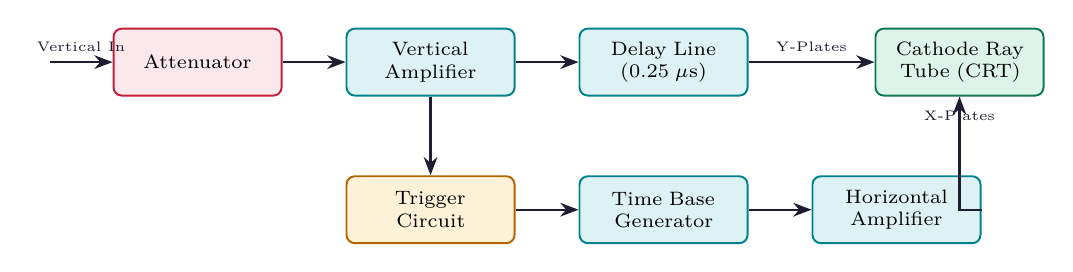
\begin{tikzpicture}[node distance=0.5cm and 0.8cm, thick, font=\small,
  sblock/.style={rectangle, draw=myteal, fill=hdrteal, text width=1.9cm,
    align=center, minimum height=0.85cm, font=\scriptsize, rounded corners=3pt, line width=0.7pt},
  sred/.style={rectangle, draw=myred, fill=hdrred, text width=1.9cm,
    align=center, minimum height=0.85cm, font=\scriptsize, rounded corners=3pt, line width=0.7pt},
  samber/.style={rectangle, draw=myamber, fill=hdramber, text width=1.9cm,
    align=center, minimum height=0.85cm, font=\scriptsize, rounded corners=3pt, line width=0.7pt},
  sgreen/.style={rectangle, draw=mygreen, fill=hdrgreen, text width=1.9cm,
    align=center, minimum height=0.85cm, font=\scriptsize, rounded corners=3pt, line width=0.7pt}]

  % Vertical Channel
  \node[sred] (att) {Attenuator};
  \node[sblock, right=of att] (vamp) {Vertical\\Amplifier};
  \node[sblock, right=of vamp] (delay) {Delay Line\\(0.25 $\mu$s)};
  
  % CRT Block
  \node[sgreen, right=1.6cm of delay] (crt) {Cathode Ray\\Tube (CRT)};

  % Horizontal Channel
  \node[samber, below=1.0cm of vamp] (trig) {Trigger\\Circuit};
  \node[sblock, right=of trig] (tb) {Time Base\\Generator};
  \node[sblock, right=of tb] (hamp) {Horizontal\\Amplifier};

  % Paths
  \draw[arrow] ($(att.west) - (0.8, 0)$) -- node[above, font=\tiny] {Vertical In} (att.west);
  \draw[arrow] (att) -- (vamp);
  \draw[arrow] (vamp) -- (delay);
  \draw[arrow] (delay) -- node[above, font=\tiny] {Y-Plates} (crt.west);
  
  \draw[arrow] (vamp.south) -- (trig.north);
  \draw[arrow] (trig) -- (tb);
  \draw[arrow] (tb) -- (hamp);
  \draw[arrow] (hamp) -| node[above, pos=0.85, font=\tiny] {X-Plates} (crt.south);
\end{tikzpicture}
\tcbset{breakable}
\end{tcolorbox}

\subsection{Key Functional Units}
\begin{itemize}[leftmargin=*, itemsep=3.5pt]
  \item \textbf{Cathode Ray Tube (CRT):} The heart of the CRO. Contains an electron gun (produces a focused electron beam), deflection plates (Y-plates for vertical input, X-plates for horizontal sweep), and a phosphor screen that glows when struck by electrons.
  \item \textbf{Delay Line:} Placed in the vertical channel. Since the trigger circuit and time-base generator require about $0.25\,\mu\text{s}$ to activate and generate the horizontal sweep, the vertical signal must be delayed by this duration. This ensures the sweep starts exactly when the signal begins, preventing the display from losing the leading edge.
  \item \textbf{Time Base Generator:} Generates a \textbf{saw-tooth ramp voltage} that sweeps the electron beam horizontally across the screen at a constant velocity, creating a linear time scale.
\end{itemize}

% ===============================================================================
\section{Lissajous Figures}
% ===============================================================================

When two sine waves are applied simultaneously to the horizontal and vertical deflection plates without the time base active, the resulting pattern on the screen is called a \textbf{Lissajous Figure}. It is used to measure phase difference and frequency.

\begin{tcolorbox}[formulabox, title={\textbf{Lissajous Wave Measurements}}]
\begin{enumerate}[leftmargin=*, itemsep=4.5pt, label=\arabic*.]
  \item \textbf{Phase Measurement ($\theta$):}
    For an ellipse centered at the origin, let $y_1$ be the y-intercept, and $y_2$ be the maximum vertical deflection:
    $$\sin \theta = \frac{y_1}{y_2} \implies \theta = \sin^{-1}\left(\frac{y_1}{y_2}\right)$$
    - If the major axis lies in Quadrants I \& III: $\theta$ is between $0^\circ$ and $90^\circ$ (or $270^\circ$--$360^\circ$).
    - If the major axis lies in Quadrants II \& IV: $\theta$ is between $90^\circ$ and $180^\circ$ (or $180^\circ$--$270^\circ$).
    - Circle $\implies \theta = 90^\circ$ or $270^\circ$. Straight line $\implies \theta = 0^\circ$ or $180^\circ$.
  \item \textbf{Frequency Measurement ($f_x, f_y$):}
    Let $N_h$ be the number of horizontal tangencies (intersections with a horizontal line at top), and $N_v$ be the number of vertical tangencies:
    $$\frac{f_y}{f_x} = \frac{N_h}{N_v} \implies f_y = f_x \cdot \frac{N_h}{N_v}$$
\end{enumerate}
\end{tcolorbox}

% ===============================================================================
\section{DSO \& Special Purpose Oscilloscopes}
% ===============================================================================

\subsection{Digital Storage Oscilloscope (DSO)}
A \textbf{DSO} digitizes, processes, and stores incoming signals in RAM before displaying them. 
- \textbf{Signal Flow:} Input signal $\to$ Attenuator $\to$ Sample \& Hold circuit $\to$ Analog-to-Digital Converter (ADC) $\to$ Digital memory (RAM) $\to$ Microprocessor $\to$ DAC / Display.
- \textbf{Advantages:} Permanent storage, pre-trigger viewing (displays signals before trigger event), mathematical processing (FFT, RMS, average), and easy data export.

\subsection{Dual Trace vs. Dual Beam CRO}
To display two channels on a screen:
\begin{itemize}[leftmargin=*, itemsep=3.5pt]
  \item \textbf{Dual Trace CRO:} Uses a single electron gun and single set of deflection plates. An electronic switch alternates rapidly between Channel A and B:
    - \textbf{Alternate Mode:} Displays one full sweep of Channel A, then one full sweep of Channel B. Best for high frequencies.
    - \textbf{Chop Mode:} Rapidly switches between A and B at a frequency of $\approx 100\,\text{kHz}$ during a single sweep. Best for low-frequency signals.
  \item \textbf{Dual Beam CRO:} Uses a special CRT with \textbf{two independent electron guns} and two sets of vertical deflection plates. Both signals are projected simultaneously. Extremely expensive but has no switching lag.
\end{itemize}

\newpage
% ===============================================================================
% MANDATORY QUICK REVISION PAGE
% ===============================================================================
\begin{center}
  {\large\bfseries\color{myred} Quick Revision --- Module 3}\\[3pt]
  {\small\color{mydark} Oscilloscopes (CRO \& DSO) $|$ OE-EC604A}
\end{center}
\noindent{\color{myred}\rule{\linewidth}{1.2pt}}
\vspace{4pt}

\begin{tcolorbox}[formulabox, title={\textbf{Key Oscilloscope Equations}}]
$$\text{Lissajous Phase Difference:} \quad \theta = \sin^{-1}\left(\frac{y_1}{y_2}\right)$$
$$\text{Frequency Calculation:} \quad \frac{f_y}{f_x} = \frac{N_{\text{tangencies\_horizontal}}}{N_{\text{tangencies\_vertical}}}$$
$$\text{CRO Probe Attenuation:} \quad v_{\text{in}} = v_{\text{scope}} \left(1 + \frac{R_{\text{probe}}}{R_{\text{scope}}}\right)$$
\end{tcolorbox}

\begin{tcolorbox}[defbox, title={\textbf{One-Line Definitions}}]
\begin{itemize}[leftmargin=*, itemsep=2.5pt, topsep=0pt]
  \item \textbf{Delay Line:} Coaxial cable delaying vertical signal to align with sweep startup trigger.
  \item \textbf{Time Base Circuit:} Generator producing saw-tooth sweep voltage to move beam linearly across horizontal axis.
  \item \textbf{Lissajous Pattern:} Figure generated on scope screen when two sine waves are fed to X and Y deflection plates.
  \item \textbf{Dual Trace:} Scope using single gun and electronic switch to show two signals on one screen.
  \item \textbf{DSO:} Digital Scope that samples incoming analog signals, converts them to digital data, and stores them in RAM.
  \item \textbf{10x Probe:} Passive attenuating probe containing a $9\,\text{M}\Omega$ resistor to increase input impedance to $10\,\text{M}\Omega$.
\end{itemize}
\end{tcolorbox}

\begin{tcolorbox}[exambox, title={\textbf{Frequently Asked / Viva Questions}}]
\begin{enumerate}[topsep=0pt, label=\textbf{Q\arabic*.}, itemsep=5pt]
  \item \Q{What is the primary purpose of the Delay Line in a CRO vertical channel?}
    The time base sweep generator requires around $0.25\,\mu\text{s}$ of processing delay to trigger after a signal arrives. If the vertical signal is fed directly to the Y-plates, it will reach the plates before the sweep starts, cutting off the leading edge of the waveform on the display. The delay line holds the vertical signal back by $0.25\,\mu\text{s}$ to synchronize it.
  \item \Q{Differentiate between Alternate Mode and Chop Mode in a Dual Trace CRO.}
    Alternate mode displays Channel A on one sweep and Channel B on the next sweep, which is suited for high-frequency signals. Chop mode switches back and forth between Channel A and B at a fast rate (e.g., $100\,\text{kHz}$) within a single sweep, making it suitable for low-frequency signals.
  \item \Q{Explain how phase difference is calculated from a Lissajous figure.}
    The phase difference is calculated using the formula $\theta = \sin^{-1}(y_1/y_2)$, where $y_1$ is the y-intercept (height where ellipse crosses vertical axis) and $y_2$ is the maximum vertical height of the ellipse.
  \item \Q{A Lissajous figure on screen has 3 horizontal tangencies and 2 vertical tangencies. The horizontal input frequency is $1\,\text{kHz}$. Calculate the vertical input frequency.}\\
    Using the tangency formula: $f_y / f_x = N_h / N_v \implies f_y / 1000 = 3 / 2$.\par
    $f_y = 1000 \times 1.5 = 1500\,\text{Hz} = 1.5\,\text{kHz}$.
  \item \Q{What are the advantages of a DSO over a conventional analog CRO?}
    A DSO can permanently store waveforms in memory, display pre-trigger signals (pre-trigger viewing), process signal data mathematically (FFT, peak detection, averaging), and export digital files directly to a computer.
  \item \Q{Explain the working of a 10x passive probe.}
    A 10x passive probe contains a $9\,\text{M}\Omega$ resistor in series with a shunt capacitor. When connected to a standard CRO channel (which has $1\,\text{M}\Omega$ input resistance), it forms a 10:1 voltage divider. This reduces the voltage reaching the scope to $1/10$th, but increases the overall input impedance to $10\,\text{M}\Omega$, minimizing circuit loading.
  \item \Q{What is the function of the phosphor coating on a CRT screen?}
    When high-energy electrons strike the phosphor coating, it fluoresces (emits visible light) and exhibits phosphorescence (continues to glow for a short duration), creating a stable trace of the electrical signal.
  \item \Q{Differentiate between Dual Trace and Dual Beam CROs.}
    Dual trace uses a single electron gun and single set of deflection plates, using switching circuits to alternate signals. Dual beam uses two independent electron guns and vertical deflection plates to project two beams simultaneously, eliminating switching lag.
  \item \Q{Explain the working of time base generator in a CRO.}
    It uses a UJT (uni-junction transistor) sweep circuit to charge a capacitor at a constant current rate, creating a linear rising ramp. Once it hits a peak, it discharges rapidly. This saw-tooth wave sweeps the beam horizontally.
  \item \Q{What is sampling in a Sampling Oscilloscope?}
    Sampling is a technique used to display extremely high-frequency signals (GHz range). The oscilloscope takes discrete amplitude samples at progressively delayed intervals over multiple successive cycles of the periodic signal, reconstructing the high-speed wave at a lower frequency.
\end{enumerate}
\end{tcolorbox}

\begin{tcolorbox}[tikzbox, title={Dual Trace vs Dual Beam Oscilloscope Comparison}]
\renewcommand{\arraystretch}{1.4}
\par\noindent
\begin{tabularx}{\linewidth}{|B{2.2cm}|>{\small\centering\arraybackslash}X|>{\small\centering\arraybackslash}X|}
\hline
\textbf{Feature} & \textbf{\color{myred}Dual Trace CRO} & \textbf{\color{myteal}Dual Beam CRO} \\
\hline
\textbf{Electron Gun} & Single electron gun. & Two independent electron guns. \\
\hline
\textbf{Deflection Plates} & Single set of vertical plates. & Two independent sets of vertical plates. \\
\hline
\textbf{Signal Display} & Time-shared switching (alt/chop). & Truly simultaneous display. \\
\hline
\textbf{Cost \& Design} & Moderate cost, simpler circuitry. & Extremely high cost, complex CRT tube. \\
\hline
\end{tabularx}
\end{tcolorbox}

\end{document}
